%%%%%%%%%%%%%%%%%%%%%%%%%%%%%%%%%%%%%%%%%%%%%%%%%%%%%%%%%%%%%%%%%
\subsubsection{Theorem 4}		%	TESTFÄLLE - RMin
%%%%%%%%%%%%%%%%%%%%%%%%%%%%%%%%%%%%%%%%%%%%%%%%%%%%%%%%%%%%%%%%%

\noindent
Nach Theorem~\ref{theo: min_4} benötigt \Rm $\mathbb{E}[\mfgm]=\mathcal{O}(\varepsilon^{-1}\log\log(n))$ Vergleiche für das Minimum und $\mathbb{E}[\mfgr]=\mathcal{O}(n^{\varepsilon})$ für alle übrigen Elemente.\\[.1cm]
Somit hat die Eingabe nun die Form $(n, n^{\varepsilon})$. Im Folgenden wird zuerst der Parameter $\varepsilon$ und anschließend der Parameter $n$ fixiert, um die Abhängigkeit zu dem jeweils anderen Parameter zu überprüfen.\\
Für die aufgeführten Experimente wurden die Parameter $n$ und $\varepsilon$ so gewählt, dass $n^{\varepsilon}$ weiterhin eine Zweierpotenz ist.\\[.15cm]

\noindent
Nun werden die Auswertungen für $\varepsilon=1/2, 1/4,\gamma$ mit $0<\gamma\ll 1/2$ diskutiert.\\
Es wurden wie auch im Anhang beiliegend weitere Werte durchlaufen, welche jedoch keine nennenswerten Unregelmäßigkeiten aufweisen.\\[.1cm]

%-- HERE
\noindent
Für $\varepsilon=1/2$ wird eine \fg von $\mathbb{E}[\mfgm]=\mathcal{O}(2\cdot\log\log(n))$ für das Minimum und $\mathbb{E}[\mfgr]=\mathcal{O}(n^{1/2})$ für alle übrigen Elemente erwartet.\\
Um diese Aussage zu überprüfen, wurde der Algorithmus nun wiederholt mit dem Eingabetupel $(n', n'^{1/2})$ für die Werte $n'=2^{2\cdot i}$, $i\in \{3,\cdots,20\}$ jeweils Zehntausend mal durchlaufen.
%%%%%%%%%%%%%%%%%%%%%%%%%%%%%%%%%%%%%%%%%%%%%%%%%%%%%%%%%%%%%%%%%
%	MIN
\subsubsection*{\textit{Fragile complexity} des Minimum Elements}
Zuerst untersuchen wir die \fg des Minimums $f_{min}(n)$. 

% ---------------------------------------------------------------
%	FIG: FG Min
\begin{figure}[H]
	\hspace*{-1.1cm}
    \begin{minipage}[t]{.30\textwidth}
        \centering
		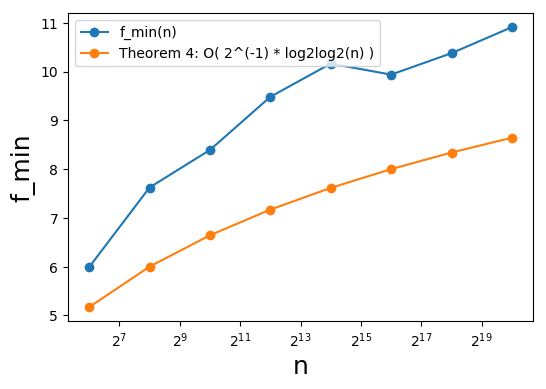
\includegraphics[width=1.075\textwidth]{pictures/min_theo4_2_min_pred.png}
    \end{minipage}
    \hspace*{0.4cm}
    \begin{minipage}[t]{.30\textwidth}
        \centering
        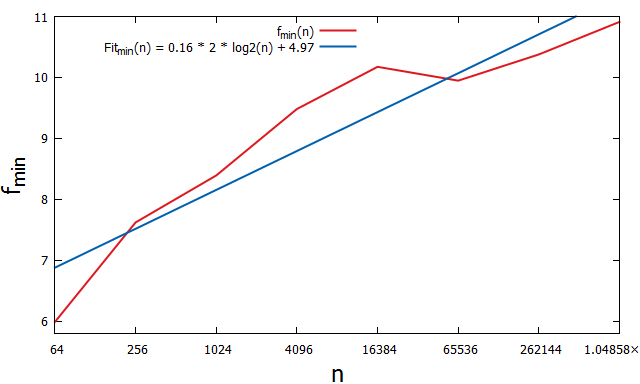
\includegraphics[width=1.21\textwidth]{pictures/min_theo4_2_fit_min_log.png}
    \end{minipage}
    %
    \hspace*{0.85cm}
	%    
    \begin{minipage}[t]{.30\textwidth}
        \centering
        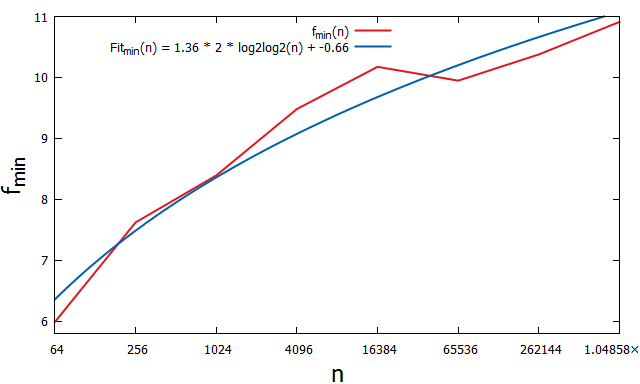
\includegraphics[width=1.21\textwidth]{pictures/min_theo4_2_fit_min_loglog.png}
    \end{minipage}
    \vspace*{-.1cm}
    \captionof{figure}{(Skalierter) Vorhersage und Fit für $f_{min}(n)$ mit $k(n)=n^{1/2}$.}\label{fig: min_theo4_fit_min}
\end{figure}

% ---------------------------------------------------------------
\noindent
Wie im ersten Bild der Abbildung~\ref{fig: min_theo4_fit_min} zu sehen wurde die aus Theorem~\ref{theo: min_4} stammende Abschätzung ohne weitere Parametrisierung in ein Koordinatensystem eingetragen. Abgesehen von einer leichten Verschiebung stimmen die Bilder der Funktionen gut überein. Im mittleren Bild wird eine einfach-logarithmischer Abschätzung dargestellt. Wie jedoch nach dem logarithmischen Skalieren der $X$-Achse zu sehen ist, weist $f_{min}(n)$ weiterhin eine kurvenförmige Darstellung auf, womit der einfach-logarithmische Fall nahezu ausgeschlossen werden kann.\\[.1cm]
In der Praxis wurde sowohl ein Fit der Form $F_{min}^1(n)= a \cdot \varepsilon^{-1}\cdot \log_2(n) + b = a \cdot 2\cdot\log_2(n) + b$ als auch ein Fit der Form $F_{min}^1(n)= a \cdot 2\cdot\log_2\log_2(n) + b$ mit Startwerten $a=1$ und $b=0.001$ versucht. Es ergab sich folgende Gegenüberstellung beider Fits:

\begin{center}
\begin{tabular}{c||l|l|l|l}

&\multicolumn{1}{c|}{Param $a$}&
\multicolumn{1}{c|}{Param $b$}&
\multicolumn{1}{c|}{Sum Res}&
\multicolumn{1}{c}{$\Delta$ Last Iter}\\
\hline
$F_V^1(k)$:&$0.1595$&$4.9664$&$2.1959$&$-2.03746e-09$\\
\hline
$F_V^2(k)$:&$1.3571$&$-0.6563$&$0.7404$&$-1.34947e-13$

\end{tabular}
\end{center}

\noindent
Die Tatsache, dass der Parameter $b$ im einfach-logarithmischen Fall um den Faktor $7.57$ weiter von $0$ entfernt konvergiert ist als der doppelt-logarithmische, zusammen mit der deutlich höheren Summe der Residuenquadrate lassen den Schluss zu, dass die Vorhersage des Theorems für die \fg des Minimums \fgm auch in der Praxis bestätigt werden kann.

%%%%%%%%%%%%%%%%%%%%%%%%%%%%%%%%%%%%%%%%%%%%%%%%%%%%%%%%%%%%%%%%%
%	Rem
\subsubsection*{\textit{Fragile complexity} aller nicht-Minimum Elemente}
Nun wird die \fg aller übrigen Elemente $f_{rem}(n)$ untersucht. Theorem~\ref{theo: min_4} prognostiziert in diesem Fall eine \fg von $\mO(n^{\varepsilon})$. Vergleicht man die experimentell gemessenen Werte für  $f_{rem}(n)$ mit dem Term $n^{\varepsilon}$ bei gleicher Parametrisierung, so ergibt sich eine nahezu perfekte Übereinstimmung. Aus diesem Grund wurde in diesem Fall auf einen Fit verzichtet.\\[.1cm]

\noindent
Wie in Abbildung~\ref{fig: min_theo4_fit_rem} ebenfalls zu sehen wird die in Theorem~\ref{theo: min_3} prognostizierte Linearität der Arbeit $w(n)$ exakt eingehalten. Abschließend sei noch bemerkt, dass der Algorithmus erst ab einer Mächtigkeit der Eingabemenge $\log_2(n)=10$ den ersten rekursiven Aufruf tätigt.


% ---------------------------------------------------------------
%	FIG: FG Min
\begin{figure}[H]
	\hspace*{-1.1cm}
    \begin{minipage}[t]{.30\textwidth}
        \centering
        \raisebox{0.05cm}{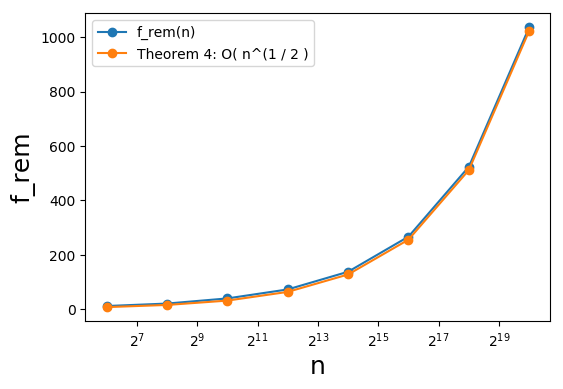
\includegraphics[width=1.21\textwidth]{pictures/min_theo4_2_rem_pred.png}
        \vspace*{.05cm}}
    \end{minipage}
    \hspace*{.8cm}
    \begin{minipage}[t]{.30\textwidth}
        \centering
        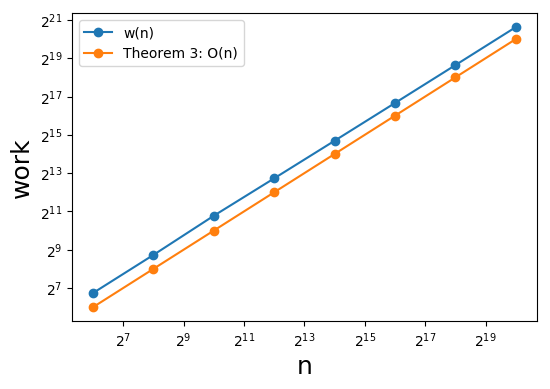
\includegraphics[width=1.2\textwidth]{pictures/min_theo4_2_work.png}
    \end{minipage}
    \hspace*{.8cm}
    \begin{minipage}[t]{.30\textwidth}
        \centering
        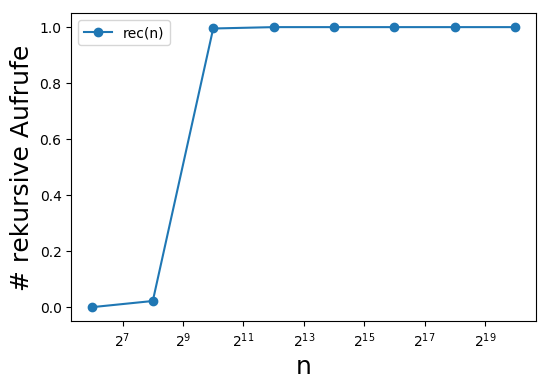
\includegraphics[width=1.21\textwidth]{pictures/min_theo4_2_rec.png}
    \end{minipage}
    \vspace*{-.1cm}
    \captionof{figure}{Vorhersage für $f_{rem}(n)$, $w(n)$ und $rec(n)$ mit $k(n)=n^{1/2}$.}\label{fig: min_theo4_fit_rem}
\end{figure}


%%%%%%%%%%%%%%%%%%%%%%%%%%%%%%%%%%%%%%%%%%%%%%%%%%%%%%%%%%%%%%%%%